\documentclass[aspectratio=169]{beamer}
\usepackage[utf8]{inputenc}
\usepackage{hyperref}
\usepackage{amsmath,amsfonts,amsthm,bm}
\usepackage{color}
\usepackage{graphicx} % Allows including images
\usepackage{subcaption}
\usepackage{booktabs} % Allows the use of \toprule, \midrule and \bottomrule in tables
\usepackage{tikz}
\usepackage{color}
\usepackage{minted}
\usetikzlibrary{automata,positioning,shapes.geometric,shapes.misc,arrows}
%\usepackage{pgfplots}
\usepackage{listings}
\usepackage{courier}
\usepackage[version=4]{mhchem}
\usepackage{array}
\usepackage{physics}

\lstset{ %
    basicstyle=\scriptsize\ttfamily, % fonts that are used for the code
    breakatwhitespace=false,         % sets if automatic breaks should only happen at whitespace
%breaklines=true,                 % sets automatic line breaking
%captionpos=b,                    % sets the caption-position to bottom
    commentstyle=\color{gray}\textit,    % comment style
    keepspaces=true,                 % keeps spaces in text, useful for keeping indentation of code (possibly needs columns=flexible)
    keywordstyle=\color{blue},       % keyword style
    language=Python,                 % the language of the code
%otherkeywords={*,...},          % if you want to add more keywords to the set
    rulecolor=\color{black},         % if not set, the frame-color may be changed on line-breaks within not-black text (e.g. comments (green here))
    showspaces=false,                % show spaces everywhere adding particular underscores; it overrides 'showstringspaces'
    showstringspaces=false,          % underline spaces within strings only
    showtabs=false,                  % show tabs within strings adding particular underscores
    stringstyle=\color{red}, % string literal style
    tabsize=4,                       % sets default tabsize to 2 spaces
    columns=fixed                    % Using fixed column width (for e.g. nice alignment)
}

\hypersetup{
    colorlinks=true,
    linkcolor=red,
    filecolor=magenta,
    urlcolor=red,
}

\DeclareMathOperator*{\argmax}{argmax}
\DeclareMathOperator*{\argmin}{argmin}
\let \vec \mathbf

\newcommand{\classname}{NANO266}
\newcommand{\classyear}{Fall 2024}
\mode<presentation> {
    \usetheme{CambridgeUS}
    \setbeamertemplate{footline}[text line]{%
        \parbox{\linewidth}{\vspace*{-8pt}\classname\hfill\classyear\hfill\insertpagenumber}}

    %\setbeamertemplate{footline}[page number]
    \setbeamertemplate{navigation symbols}{}
}


\title[\classname Temperature]{\classname~- Quantum Mechanical Modeling of Materials and Nanostructures\\Temperature}

\author{Shyue Ping Ong}
\institute[UCSD]{University of California, San Diego\\
\medskip
}
\date{\classyear} % Date, can be changed to a custom date

\begin{document}


    \begin{frame}
        \titlepage % Print the title page as the first slide
    \end{frame}

    \begin{frame}{What is Temperature?}
        Temperature is a measure of ``excess'' energy above the ground state due to excitations.

        \begin{figure}
            \centering
            \begin{subfigure}{0.45\textwidth}
                \centering
                \includegraphics[width=0.5\linewidth]{figures/10_vibrational.png}
                \caption{Vibrational}
            \end{subfigure}
            \begin{subfigure}{0.45\textwidth}
                \centering
                \includegraphics[width=0.7\linewidth]{figures/10_configurational.png}
                \caption{Configurational}
            \end{subfigure}
            \begin{subfigure}{0.45\textwidth}
                \centering
                \includegraphics[width=0.5\linewidth]{figures/10_electronic.png}
                \caption{Electronic}
            \end{subfigure}
            \begin{subfigure}{0.45\textwidth}
                \centering
                \includegraphics[width=0.7\linewidth]{figures/10_conformational.png}
                \caption{Conformational}
            \end{subfigure}
            \label{fig}
        \end{figure}

    \end{frame}

    \begin{frame}{Approximating Temperature}
        \begin{columns}
            \column{0.5\textwidth}
            Temperature changes oxygen chemical potential $\mu_{O_2}$:
            \begin{eqnarray*}
                \mu_{O_2}(T, p_{O_2}) & = & \mu_{O_2}(T, p_{O_2}^0)+ kT \ln \frac{p_{O_2}}{p_{O_2}^0}
            \end{eqnarray*}

            where $p_{O_2}$ is the partial pressure of oxygen.\newline
            \newline
            For a reaction involving only solid phases and oxygen gas, the relevant thermodynanic potential is the grand potential:\cite{ongLiFeO22008}

            \begin{eqnarray*}
                \phi & = & E - TS + PV - \mu_{O_2} N_{O_2}\\
                & \approx & E - \mu_{O_2} N_{O_2}
            \end{eqnarray*}

            \column{0.5\textwidth}

            \begin{figure}
                \centering
                \begin{subfigure}{0.47\textwidth}
                    \centering
                    \includegraphics[width=\linewidth]{lectures/figures/10_LFP_PD.png}
                \end{subfigure}
                \begin{subfigure}{0.47\textwidth}
                    \centering
                    \includegraphics[width=\linewidth]{lectures/figures/10_LFP_PD2.png}
                \end{subfigure}
            \end{figure}
        \end{columns}
    \end{frame}

    \begin{frame}{Vibrational Entropy}
        Phonons are the collective excitation in a periodic, elastic arrangement of atoms or molecules in condensed matter, like solids and some liquids.
        \begin{itemize}
            \item \textbf{Acoustic phonons} are coherent movements of atoms of the lattice out of their equilibrium positions.
            \item \textbf{Optical phonons} are out-of-phase movements of the atoms in the lattice.
        \end{itemize}

        \begin{figure}
            \centering
            \includegraphics[width=0.4\linewidth]{lectures/figures/10_Phonons.jpeg}
        \end{figure}

    \end{frame}

    \begin{frame}{Lattice Dynamics of a Monoatomic 1D Lattice}
        \begin{figure}
            \centering
            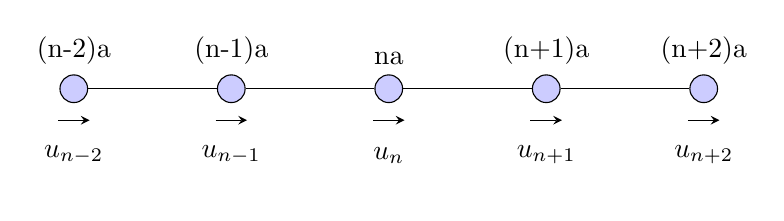
\begin{tikzpicture}[
                atom/.style={circle,draw=black,fill=white!80!blue,minimum size=10},
            ]
                \node[atom,label=(n-2)a] (1) at (2,0) { };
                \node[atom,label=(n-1)a] (2) at (4,0) { };
                \node[atom,label=na] (3) at (6,0) { };
                \node[atom,label=(n+1)a] (4) at (8,0) { };
                \node[atom,label=(n+2)a] (5) at (10,0) { };
                \draw [-stealth](1.8,-0.4) -- (2.2,-0.4);
                \draw [-stealth](3.8,-0.4) -- (4.2,-0.4);
                \draw [-stealth](5.8,-0.4) -- (6.2,-0.4);
                \draw [-stealth](7.8,-0.4) -- (8.2,-0.4);
                \draw [-stealth](9.8,-0.4) -- (10.2,-0.4);

                \node[label=$u_{n-2}$] at (2, -1.2) { };
                \node[label=$u_{n-1}$] at (4, -1.2) { };
                \node[label=$u_{n}$] at (6, -1.2) { };
                \node[label=$u_{n+1}$] at (8, -1.2) { };
                \node[label=$u_{n+2}$] at (10, -1.2) { };

% These draw commands are working as intended.
                \draw (1) -- (2);
                \draw (2) -- (3);
                \draw (3) -- (4);
                \draw (4) -- (5);
            \end{tikzpicture}
        \end{figure}
        \begin{eqnarray*}
            E(\{u_n\}) & = &  E_0(0) + \sum_n \left( \frac{\partial E}{\partial u_n} \right)_0 u_n + \frac{1}{2} \sum_{n,n'} \left( \frac{\partial^2 E}{\partial u_n \partial u_n'} \right)_0 u_n u_n' \\
            & & + \frac{1}{3!} \sum_{n,n',,n''} \left( \frac{\partial^3 E}{\partial u_n \partial u_n' \partial u_n''} \right)_0 u_n u_n' u_n'' + ...
        \end{eqnarray*}

        Truncating at 2nd derivative $\rightarrow$ Harmonic approximation

    \end{frame}


    \begin{frame}{Direct Approach - ``Frozen'' Phonons}
        Explicitly calculate the forces between every atom and construct the force constant matrix of the crystal, and hence calculate normal modes of at any particular wavevector, $\vec{q}$. \newline
        \newline

        Forces can be obtained in DFT using Hellman-Feynman Theorem.\newline
        \newline
        Pros:
        \begin{itemize}
            \item No specialized code required (except for automating displacements, etc.)
            \item Faster than linear response method, especially for reasonably sized systems.
            \item Many existing codes to help automate such computations: Phonopy, GoBaby, etc.
            \item Higher order anharmonic terms can be obtained relatively easily.
        \end{itemize}

        Cons:
        \begin{itemize}
            \item Large supercells are needed to accurately calculate the force constant matrix.
        \end{itemize}

    \end{frame}

    \begin{frame}{Linear Response Method – Density Functional Perturbation Theory (DFPT)}

        From the Hellman-Feynman Theorem, we have:
        \begin{eqnarray*}
            \frac{\partial E}{\partial \lambda_i} & = & \int \frac{\partial V_{\lambda}(\vec{r})}{\partial \lambda_i} n(\vec{r}) d\vec{r}, \frac{\partial^2 E}{\partial \lambda_i \partial \lambda_j} = \int \frac{\partial^2 V_{\lambda}(\vec{r})}{\partial \lambda_i \partial \lambda_j} n(\vec{r}) d\vec{r} + \int \frac{\partial V_{\lambda}(\vec{r})}{\partial \lambda_i } \frac{ \partial n(\vec{r}) }{\partial \lambda_j} d\vec{r}\\
        \end{eqnarray*}

        Linearizing the electron density, we get:\cite{baroniPhononsRelatedCrystal2001}

        \begin{equation*}
            \Delta n(\vec{r}) = 4 \mathrm{Re} \sum_{n=1}^{N/2} \psi_n^*(\vec{r}) \Delta \psi_n(\vec{r})
        \end{equation*}
    \end{frame}

    \begin{frame}{Linear Response Method – Density Functional Perturbation Theory (DFPT)}

        From first order perturbation theory, we have

        \begin{equation*}
        (H_{SCF} - \varepsilon_n)
            \ket{\Delta \psi_n} = -(\Delta V_{SCF}(\vec{r})-\Delta \varepsilon_n) \ket{\Delta \psi_n}
        \end{equation*}

        where

        \begin{equation*}
            \Delta V_{SCF}(\vec{r}) = -\Delta V(\vec{r}) + e^2 \int \frac{ \Delta n(\vec{r}'}{|\vec{r}-\vec{r'}|} d \vec{r'} + \frac{\partial V_{xc}}{\partial n} \Delta n(\vec{r})
        \end{equation*}

    \end{frame}

    \begin{frame}{Pros and Cons of DFPT}
        Pros:
        \begin{itemize}
            \item Can calculate phonon frequencies at arbitrary wave vectors $\vec{q}$ without use of supercells!
            \item Scaling with range of interatomic force constants is much more favorable.
        \end{itemize}

        Cons:
        \begin{itemize}
            \item Requires specialized codes.
            \item Cost of calculations typically higher than frozen phonons approach.
        \end{itemize}

    \end{frame}


    \begin{frame}{Lattice dynamics properties from DFT}

        \begin{columns}
            \column{0.5\textwidth}

            \begin{figure}
                \centering
                \begin{subfigure}{\textwidth}
                    \centering
                    \includegraphics[width=0.4\linewidth]{lectures/figures/10_Phonon_Diamond.png}
                    \caption{Phonon dispersion relations for diamond.\cite{gonzeFirstprincipleStudiesLattice2005}}
                \end{subfigure}
                \begin{subfigure}{\textwidth}
                    \centering
                    \includegraphics[width=0.3\linewidth]{lectures/figures/10_Heat_capacities.png}
                    \caption{Heat capacities as a function of temperature. The solid, dashed, and dashed-dotted curves denote CP of \ce{Ti3SiC2}, \ce{Ti3AlC2}, and \ce{Ti3GeC2}, respectively.\cite{togoFirstprinciplesPhononCalculations2010}}
                \end{subfigure}
            \end{figure}

            \column{0.5\textwidth}
            \begin{figure}
                \centering
                \includegraphics[width=0.45\linewidth]{lectures/figures/10_Phonon_Semiconductors.png}
                \caption{Calculated phonon dispersions and densities of states for binary semiconductors GaAs, AlAs, GaSb, and AlSb.\cite{baroniPhononsRelatedCrystal2001}}

            \end{figure}

        \end{columns}

    \end{frame}

    \begin{frame}{Electronic Entropy}
        Independent one-electron eigenstates can be occupied or not. Probability is given by the Fermi dirac function.
        \begin{equation*}
            f_i = \frac{e^{-\frac{\varepsilon_i-\varepsilon_f}{k_BT}}}{1+e^{--\frac{\varepsilon_i-\varepsilon_f}{k_BT}}}
        \end{equation*}

        The electronic entropy is given by:

        \begin{equation*}
            S_{elec} = -k_b \sum_i \left[ f_i \ln(f_i) + (1-f_i) \ln(1-f_i)\right]
        \end{equation*}

        \begin{itemize}
            \item Free-electron-like metals, e.g., alkali metals, have low electronic entropies due to their low density of states at the Fermi level.
            \item Transition metals have large electronic entropies because their flat $d$-bands are close to the Fermi level.
            \item Insulators generally have low electronic entropies due to the presence of a band gap.
        \end{itemize}
    \end{frame}

    \begin{frame}{Configurational Entropy}

        \begin{columns}
            \column{0.6\textwidth}
            Ising model

            \begin{equation*}
                H(\sigma) = -\sum_{i,j} J_{ij} \sigma_i \sigma_j + \mu \sum_i h_i \sigma_i
            \end{equation*}

            \begin{itemize}
                \item $J_{ij} > 0$ $\implies$ Ferromagnetic ground state.
                \item $J_{ij} < 0$ $\implies$ Anti-ferromagnetic ground state (see right picture).
                \item System is permanently magnetized at low temperatures.
                \item At Curie temperature, $T_c$, phase transition occurs between magnetic and paramagnetic phases (net magnetization is zero).
            \end{itemize}
            

            \column{0.4\textwidth}
            \begin{figure}
                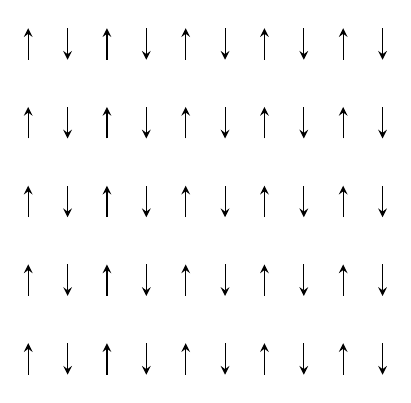
\begin{tikzpicture}[scale=0.5]
                    \foreach \i in {0,...,4}
                        {
                        \foreach \j in {0,...,4}
                            {
                            \draw [-stealth](2*\i,2*\j-0.4) -- (2*\i,2*\j+0.4);
                            \draw [stealth-](2*\i+1,2*\j-0.4) -- (2*\i+1,2*\j+0.4);
                        }
                    }
                \end{tikzpicture}
            \end{figure}

        \end{columns}
    \end{frame}


    \begin{frame}{Cluster Expansion - Generalization of Ising Model}

\begin{columns}
\column{0.4\textwidth}
\begin{figure}
            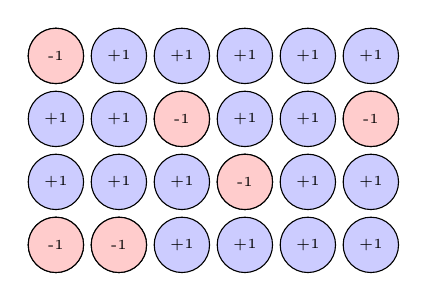
\begin{tikzpicture}[
                scale=0.4,
                atom/.style={circle,draw=black,fill=white!80!blue,minimum size=20},
                dopant/.style={circle,draw=black,fill=white!80!red,minimum size=20}
            ]
                \foreach \i in {1,...,6}
                    {
                    \foreach \j in {1,...,4}
                        {
                        \node[atom] (\i\j) at (2*\i,2*\j) { \tiny{+1}};
                    }
                }
                \node[dopant] ( a ) at (2,2) {\tiny{-1} };
                \node[dopant] ( b ) at (4,2) {\tiny{-1}};
                \node[dopant] ( c ) at (8,4) {\tiny{-1} };
                \node[dopant] ( d ) at (12, 6) {\tiny{-1} };
                \node[dopant] ( a ) at (6,6) {\tiny{-1} };
                \node[dopant] ( a ) at (2, 8) {\tiny{-1} };
            \end{tikzpicture}
            \caption{Spin variables ($\sigma = \pm 1$) represent atomic species instead of magnetism. }
         \end{figure}
\column{0.6\textwidth}
\begin{equation*}
            H(\{\sigma\}) = V_0 + \sum_{i,j} V_{ij} \sigma_i \sigma_j + + \sum_{i,j,k} V_{ijk} \sigma_i \sigma_j \sigma_k + ...
        \end{equation*}
                \begin{itemize}
            \item Expansion based on 2-body, 3-body, ..., n-body interactions.
            \item $V_{ij}$, $V_{ijk}$, etc. are known as effective cluster interactions (ECIs) and fitted by regression or machine learning from DFT calculations of different configurations $\{\sigma\}$.
        \end{itemize}

\end{columns}

    \end{frame}


    \begin{frame}{Monte Carlo (MC) Simulations}
        Partition function

        \begin{equation*}
            Z = \sum_{\{\sigma\}} e^{-\frac{E[\{\sigma\}]}{k_BT}}
        \end{equation*}

        Sample states of a system stochastically with probabilities $p$ that match those expected physically to obtain thermodynamic averages:
        \begin{eqnarray*}
            \left< A \right> & = & \int_{\{\sigma\}} A_{\{\sigma\}} p(\{\sigma\}) d \{\sigma\}\\
            & = & \sum_{\{\sigma\}} A_{\{\sigma\}} \frac{e^{-\frac{E[\{\sigma\}]}{k_BT}}}{Z}
        \end{eqnarray*}

    \end{frame}

    \begin{frame}{Simple versus Importance Sampling}

        Simple sampling (random choice of states) is inefficient because thermodynamic probabilities are very sharply peaked (exponential term)!

        \begin{figure}
            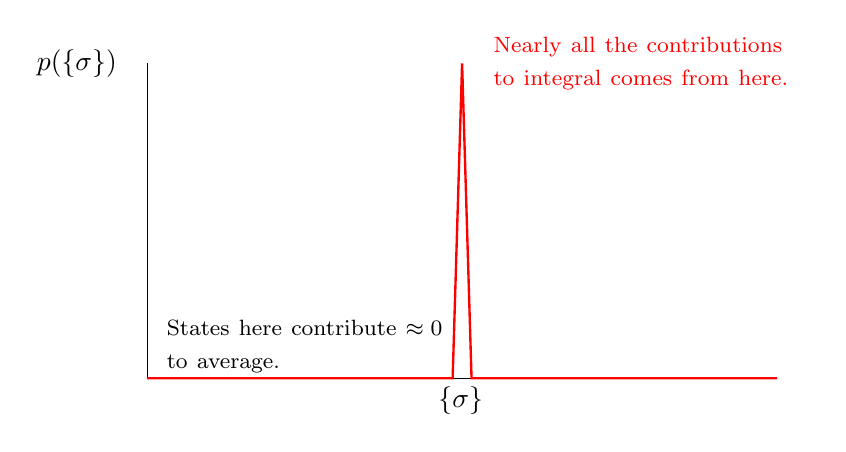
\begin{tikzpicture}[scale=0.4]
                \draw [-] (0,0) -- (0,10);
                \draw [-] (0,0) -- (20,0);
                \draw [-,color=red,line width=0.3mm] (0,0) -- (9.7,0) -- (10, 10) -- (10.3, 0) -- (20, 0);
                \node[text width=2cm] at (-1,10) {$p(\{\sigma\})$};
                \node[text width=1cm] at (10.5,-0.7) {$\{\sigma\}$};
                \node[text width=3.5cm] at (5,1) {\footnotesize{States here contribute $\approx 0$ to average.}};
                \node[text width=4cm,color=red] at (16,10) {\footnotesize{Nearly all the contributions to integral comes from here.}};
            \end{tikzpicture}
        \end{figure}

    \end{frame}

    \begin{frame}{Detailed balance}
        At steady state, flux between two states must be equal, i.e.,

        \begin{equation*}
            p(m) \pi(m \rightarrow n) = p(n) \pi(n \rightarrow m)
        \end{equation*}

        where $\pi(m \rightarrow n)$ is the transition matrix given by $a(m \rightarrow n)A(m \rightarrow n)$ where $a$ is the attempt distribution and $A$ is the acceptance distribution. If the attempt distributions are symmetric ($a(m \rightarrow n) = a(n \rightarrow m)$), i.e., random selection,
        \begin{eqnarray*}
            p(m) A(m \rightarrow n) & = & p(n) A(n \rightarrow m)\\
            \frac{A(m \rightarrow n)}{A(n \rightarrow m)} & = & \frac{p(n)}{p(m)} = e^{-\frac{E_n - E_m}{k_BT}}
        \end{eqnarray*}

        So we set
        \begin{eqnarray*}
            A(m \rightarrow n) = \begin{cases}
                                     e^{-\frac{E_n - E_m}{k_BT}} &p(n) < p(m)\\
                                     1 & p(n) > p(m)\\
            \end{cases}
        \end{eqnarray*}

    \end{frame}

    \begin{frame}{Metropolis Algorithm}

    \begin{columns}
\column{0.4\textwidth}
\begin{figure}
            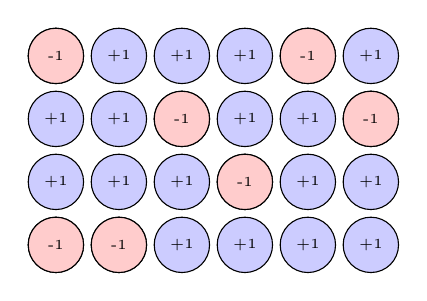
\begin{tikzpicture}[
                scale=0.4,
                atom/.style={circle,draw=black,fill=white!80!blue,minimum size=20},
                dopant/.style={circle,draw=black,fill=white!80!red,minimum size=20}
            ]
                \foreach \i in {1,...,6}
                    {
                    \foreach \j in {1,...,4}
                        {
                        \node[atom] (\i\j) at (2*\i,2*\j) { \tiny{+1}};
                    }
                }
                \node[dopant] ( a ) at (2,2) {\tiny{-1} };
                \node[dopant] ( b ) at (4,2) {\tiny{-1}};
                \node[dopant] ( c ) at (8,4) {\tiny{-1} };
                \node[dopant] ( d ) at (12, 6) {\tiny{-1} };
                \node[dopant] ( a ) at (6,6) {\tiny{-1} };
                \node[dopant] ( a ) at (2, 8) {\tiny{-1} };
                \pause
                \node[dopant] ( flip ) at (10,8) { \tiny{-1}};
            \end{tikzpicture}
        \end{figure}
\column{0.6\textwidth}
\begin{enumerate}
            \item Start in state $\{\sigma_1, \sigma_2,.., \sigma_n\}$.
            \item Choose a new set of spins by ``flipping'' randomly selected $\sigma_i^* = - \sigma_i$
            \item Calculate $\Delta E = E(\{\sigma_1, \sigma_2,..-\sigma_i,..., \sigma_n\}) - E(\{\sigma_1, \sigma_2,..\sigma_i,..., \sigma_n\})$.
            \item If $\Delta E < 0$, accept $\sigma_i^*$. If $\Delta E > 0$, accept $\sigma_i^*$ with probability $e^{-\beta \Delta E}$.
            \item Go back to step 1.
        \end{enumerate}
\end{columns} 
        

        

    \end{frame}

    \begin{frame}{Example: Temperature-dependent phase diagram of \ce{Na_xCoO2}}
        \begin{figure}
            \centering
            \begin{subfigure}{0.55\textwidth}
                \centering
                \includegraphics[width=\linewidth]{lectures/figures/10_NCO_PD.png}
                \caption{GGA convex hull of \ce{Na_xCoO2}. (b)–(j): In-plane ordering of the GGA ground states at $x = 0.5, 0.56, 0.6, 0.67, 0.71, 0.77, 0.81, 0.84, 0.86$.}
            \end{subfigure}
            \begin{subfigure}{0.4\textwidth}
                \centering
                \includegraphics[width=\linewidth]{lectures/figures/10_NCO_CE_PD.png}
                \caption{GGA phase diagram obtained by MC simulation from the cluster expansion.\cite{hinumaTemperatureconcentrationPhaseDiagram2008}}
            \end{subfigure}
        \end{figure}
    \end{frame}

    \begin{frame}{State of the art in cluster expansions}

        \begin{columns}
            \column{0.5\textwidth}
            \begin{figure}
                \centering
                \includegraphics[width=\linewidth]{lectures/figures/10_compressive_sensing.png}
                \caption{Using machine learning to fit cluster expansions.\cite{nelsonCompressiveSensingParadigm2013}}
            \end{figure}
            \column{0.5\textwidth}
            \begin{figure}
                \centering
                \includegraphics[width=\linewidth]{lectures/figures/10_tensorial_CE.png}
                \caption{CE for tensorial quantitis.\cite{vandewalleCompleteRepresentationStructureproperty2008}}
            \end{figure}
        \end{columns}

    \end{frame}

    \begin{frame}[allowframebreaks]{Bibliography}
        \bibliographystyle{unsrt}
        \bibliography{refs}
    \end{frame}



    \begin{frame}
        \Huge{\centerline{The End}}
    \end{frame}

\end{document}

